% =====================================================================
% Part III -- Endogenous Coupling and Exotypes.  Draft 2026-08-06 (claude-14).
%
% Scope per Joe, 2026-08-06: Part III explains the exotype layer and reports
% what the search found AT THE END.  The EFE miner -- the apparatus that did the
% searching -- moves to a supplement: it is a tool, not a theory of MetaCAs.
% The research question is stated openly as UNANSWERED.
%
% Labels referenced here that exist in draft7.tex: sec:object, eq:prop,
% sec:classification, sec:census, sec:full-census, sec:gain, part:core.
% =====================================================================

\part{Endogenous Coupling and Exotypes}
\label{part:endogenous}

\noindent In Part~II the gain of the phenotype-to-genotype loop is a parameter we
set. This part asks what happens when it is not. It does so twice, at two
different levels of the construction. First the \emph{condition} under which a
rewriting operator fires becomes a function of the lattice rather than a dial we
turn. Then the \emph{operator itself} becomes a property of the cell rather than
of the run. The first half studies an update architecture of the Part~II kind whose firing
condition is set by the lattice; the second draws its per-cell rewriting operators from the
family Part~I classifies and lets the lattice choose among them.

\section{An Endogenous Gain}
\label{sec:endogenous-gain}

A \emph{conditional composition} applies one operator where a local predicate
holds and another where it does not. Throughout this section the first is
conservative transport at unit rate, which sits high on the
calibration of \secref{sec:causal} at $25.38$, and the second is holding, which
sits near its floor at $1.21$; the predicate decides, cell by cell and step
by step, which applies, and its \emph{firing fraction} $f$ is measured from the
run rather than prescribed. Two disciplines inherited from the gain dial of
\secref{sec:gain} make the comparison meaningful: the transport stream advances
at every opportunity whether or not the gate fires, so a phenotype-reading
predicate cannot desynchronise the branches of a damage fork; and where the
predicate consumes randomness, those draws come from a separate stream re-seeded
identically in both branches.

A gate firing at a prescribed rate, blind to the phenotype, is described across
six rates spanning $f = 0.10$ to $0.94$ by a line through the holding value,
%
\begin{equation}
  \mathrm{reach}(f) \;=\; 1.21 \;+\; 22.42\,f ,
  \label{eq:blind-line}
\end{equation}
%
with $R^{2} = 0.993$. A blind conditional composition is therefore \emph{exactly}
a gain dial, its duty cycle playing the role $\gamma$ plays in
\secref{sec:gain}. The construction adds nothing on its own; what matters is what
the condition reads.

Letting it read the phenotype changes that. Writing $\mathrm{agree}\,k/m$ for the
condition that at least $k$ cells of the centred circular $m$-cell phenotype
neighbourhood agree with the centre, thirteen such gates spanning widths
$m \in \{3,5,7,9\}$ all exceed Equation~\eqref{eq:blind-line} at their own
measured firing fraction, several by a wide margin. The widest permissive gate,
$\mathrm{agree}\,5/9$, reaches $38.23$ while firing on only $63\%$ of
opportunities --- above unit-rate transport's own $25.38$. Firing a chaotic
operator less often, in the right places, spreads damage further than firing it
always. What predicts the size of the departure is the \emph{width} of the
neighbourhood read rather than how hard the gate is to satisfy, though strictness is
nearly collinear with $f$ and the two are not cleanly separable here.

That admits a deflationary reading, and the control that rules it out is the one
that matters here. A gate reading $m$ cells has neighbouring decisions sharing
$m-1$ inputs, so width \emph{is} the spatial correlation length of the firing
pattern, and correlated firing of a transport operator composes adjacent swaps
into longer-range movement. A \emph{frozen} gate applies the identical predicate
to the phenotype as it stood at $t^{*}$: same width, same spatial statistics, a
real phenotype field, and therefore the same correlation structure --- but no
ability to track where a perturbation has since spread. Across seven pairs
matched on $(m,k)$ the live gate exceeds its frozen counterpart in every case, by
$14.5$ cells on average, and every frozen departure from the blind line is
\emph{negative}, between $-0.04$ and $-4.18$. The comparison is conservative in
the direction that matters: the frozen gate fires \emph{more} often than its live
counterpart in six of the seven pairs, and still reaches less.

The gate is therefore a targeting mechanism, and targeting works only on current
information. An endogenous gain does not escape the causal currency of what the
genotype reads; it re-derives it. A composition whose condition is blind
reproduces the dial exactly, and one whose condition reads the phenotype exceeds
it precisely to the extent that what it reads is current.

\section{From Gate to Operator}
\label{sec:exotype-intro}

The gate chooses \emph{when} an operator fires. It does not choose \emph{which}.
Throughout the preceding section the pair of constituents is fixed, and the
predicate selects between them; the permutation $\sig$ supplying the rewriting is
a property of the run. The remainder of this part removes that restriction. Each
cell carries its own propagator, drawn from a small named vocabulary and
transmitted between neighbours, so the operator acting at a site becomes part of
the local state.

\section{The Question This Part Does Not Answer}
\label{sec:exotype-question}

The motivating question is easy to state and we have not answered it. The Part~II architectures and the endogenous gate are placed on
a scale by an instrument we hold: damage reach, computed by forking the run and
perturbing a twin. The question is whether the construction can dispense with that
instrument---whether a MetaCA carrying an exotype layer can find its own operating
point using only quantities available to it at runtime. Damage reach cannot be that
quantity, since no system can fork itself; and the coordinate it measures is causal
propagation rather than dynamical regime, so it would not by itself say where the
system should arrive.

We built an apparatus to test this and it did not settle the question.
Supplement~5 documents it in full, because its negative results are specific enough to
be reusable, and because one of them bears directly on the question: a runtime-computable
pair of observables tracks an intrinsic objective well ($R^2 = 0.73$ held out) and damage
reach not at all ($R^2 = 0.02$). What the supplement does not contain is a system that
searched and found. The examples reported below were located by that apparatus together
with our own reading of what it returned, and we are not able to separate the two
contributions.

We therefore make a weaker claim, and state it plainly so that it is not
mistaken for the stronger one. \textbf{A self-driving search, had it worked,
would have been expected to return configurations with robust intermediate
behaviour. We report such configurations.} They are reported here as objects with measured properties, not
as the output of an autonomous procedure, and they establish that the targets of
such a search exist in this substrate rather than that the substrate can find
them.

\section{The Layer}
\label{sec:exotype-layer}

An \emph{exotype} is a per-cell assignment of a propagator. The vocabulary is a
set of named permutations $\sig$; the grid holds one name per site; and the
names are transmitted between neighbouring sites by a local policy. Nothing in
the vocabulary is new to this paper---each name denotes a member of the family
Equation~\eqref{eq:prop} defines---but the assignment is new, because $\sig$ has
until now been a property of a run rather than of a cell.

The transition is one elementary write. At a site whose genotype is the
eight-bit rule $g$, with $\sig$ the propagator the site currently carries, a
coordinate $k \in \{0,\dots,7\}$ is drawn uniformly at each step and
%
\begin{equation}
  g'\bigl(\sig(k)\bigr) \;=\; \neg\, g(k),
  \label{eq:exotype-write}
\end{equation}
%
with $g$ unchanged elsewhere. Comparing this with \secref{sec:object}: the
simultaneous operator $P_\sig$ applies Equation~\eqref{eq:exotype-write} at all
eight coordinates at once, and the spatial experiments of Part~I place its
elementary writes inside the two-layer automaton. The exotype layer is that same
elementary write, drawn one coordinate at a time, with $\sig$ read from the cell
rather than from the run.

Three properties of this transition are worth stating because the informal
vocabulary the project has used around it---exotype as \emph{culture},
transmissible but not heritable---obscures all three.

First, \textbf{the exotype edits the rule; it does not change how the rule is
applied.} $\sig$ never touches the propagation of phenotype state. It selects a
write address inside the genotype. The word \emph{propagator} is unhelpful on
exactly this point, and we retain it only because Part~I has established it for
the operator family.

Second, \textbf{when $\sig$ is the identity the transition is a point
mutation}---flip a uniformly chosen bit of the rule. For every $\sig$ other than
the identity the read address and the write address differ, so the operation
transfers inverted information from one entry of the truth table to another.
An exotype is therefore best described as a locally varying, structured mutation
operator, whose bias is which bit of the rule is rewritten from which.

Third, \textbf{it fires at every applied site at every step.} It is the ordinary
path, not a rare perturbation. In the configuration measured here it is also the
dominant one, though we report the split without the per-event protocol needed to audit
it.3\%$ from the policy blend.

We also drop the phrase \emph{transmissible but not heritable}. The exotype grid
persists across steps and is transmitted between sites; whatever term is
preferred, that is inheritance of an acquired modifier in the sense that a
Baldwin-style argument requires, and declining the word does not change the
causal structure. What the layer does is better conveyed by
Equation~\eqref{eq:exotype-write} than by any of these labels.

\section{The Vocabulary Is Twelve of Forty Thousand}
\label{sec:exotype-vocabulary}

The implemented vocabulary has twelve members. The family
Equation~\eqref{eq:prop} defines has $8! = 40{,}320$. The layer therefore
instantiates $0.030\%$ of the permutation core, and if the family is widened to
the arbitrary maps the 2015 implementation actually had, $12/8^8$ is
$0.00007\%$.

The twelve are drawn from the family Part~I classifies and organised along the
coordinates that classification supplies, so Part~I's theorem audits them exactly: it
predicts, without any dynamical measurement, how many rules each member cannot alter,
and the prediction agrees in all fourteen implemented cases including the two controls
that are defined but not selectable. That agreement is an audit of the vocabulary and
not a premise of anything below; no persistence result in this part depends on it.

The twelve were chosen by hand, and the reasons were not recorded. They span both cycle
parities and both ends of the fixed-point count, which is what makes the layer's
behaviour attributable to the exotype mechanism rather than to a degenerate choice of
operator, but the selection was not designed to test any hypothesis about the family.

\section{What Varies, and What Does Not}
\label{sec:exotype-scope}

The boundary on everything this part claims is set by the same table. Of the
original four propagators, \emph{why those four} has never been justified; they
were hand-picked, and the reason is not recorded. The eight additions were made
for a documented but narrow reason: the selection dynamics had collapsed onto
\texttt{collapser} because the scoring cache iterated only the four declared
names, so the objective could not select the others. Widening the vocabulary
repaired a defect in the search, and was not an attempt to cover the family.

Consequently every dynamical result reported below is measured at one point of a
$40{,}320$-member design space, chosen by hand for unrecorded reasons, and no
experiment we have run varies $\sig$ across that space. Nothing here is known to
generalise across propagators. This is not a caveat to be added at the end; it
is a boundary on what the part is entitled to claim, and it is the most
consequential limitation of the work.

It also identifies the extension with the clearest warrant. The vocabulary is
finite and small because it is a hand-written map from names to permutations;
nothing in Equation~\eqref{eq:exotype-write} requires that. Allowing $\sig$ to
range over the family---sampled, or enumerated within a cycle type, or varied
along the cycle-parity and fixed-point axes Part~I supplies---would turn a fixed
point in the design space into a coordinate, and would make Part~I's
classification available as an experimental variable rather than only as a
prediction about twelve cases. We have not done this, and we note it as an
extension rather than as work in progress.

\section{Three Examples}
\label{sec:exotype-examples}

Supplement~5 records a search over two parameters of the selection rule: the
policy precision $\beta$ and the epistemic weight $\kappa$. The search did not
become autonomous, and its objective turns out to be the wrong target. What it
did produce is a map, and on that map three configurations are worth reporting
as objects in their own right. They are what a working search would have been
expected to return.

All three are measured the same way and by a criterion the search never used.
Write a site as \emph{frozen} at time $t$ if its phenotype has been unchanged for
the preceding fifteen steps, and \emph{live} otherwise. A run is \emph{absorbing}
if it reaches a configuration it does not leave again for the remainder of the
run. These are properties of a single
trajectory, requiring no twin run and no external reference; the horizon is the
only free choice, and we report it with every number.

\subsection{The ridge from below}

At low $\beta$ the lattice is live and stays live. At $\beta = 2$, $\kappa = 0$
the frozen fraction settles at $0.040$ and remains there through $3000$ steps, on
both seeds; the same holds at $\beta = 2$, $\kappa = 0.1$ and at $\beta = 4$ for
$\kappa \in \{0, 0.1, 0.2\}$. No run in this group reaches an absorbing state.

The mechanism is not that frozen regions fail to form. They form and are then
eaten. Over the first three measurement bands at $\beta = 2$, $\kappa = 0$ the
number of frozen domains holds at ten while their mean width collapses from
$9.0$ cells to $3.8$ and then to zero. A constant count with falling width is
boundary retreat: every domain loses territory from both edges at once. Interior
dissolution would look different --- holes opening inside frozen regions would
\emph{raise} the domain count by fragmentation --- and the count never rises.
Live territory invades frozen territory at every boundary simultaneously, and
there is nothing left at the end.

\subsection{The ridge from above}

At high $\beta$ and low $\kappa$ the same contest runs the other way, and the
losing side puts up a fight worth describing. At $\beta = 32$, $\kappa = 0.1$
the lattice carries a dense branching structure through a field of static
stripes, fragmenting the frozen field as it goes: the frozen domain count
\emph{rises} from fifteen to twenty-two over the second measurement band, which
is live territory cutting frozen territory into pieces. It then loses. The
pieces merge, the count falls to two domains of width $124$, and at $t = 1046$
the configuration stops changing and does not change again before the run
ends. Every subsequent row is
byte-identical; the final pattern has density $0.500$, so this is a frozen
pattern rather than a blank sheet.

The second seed absorbs at $t = 460$, and $\beta = 64$ absorbs at $t = 881$ and
$t = 537$. The outcome is seed-robust and the timing is not: absorption time
varies by more than a factor of two at fixed parameters, so differences of that
size between neighbouring $\beta$ carry no information.

\begin{figure}[htbp]
\centering
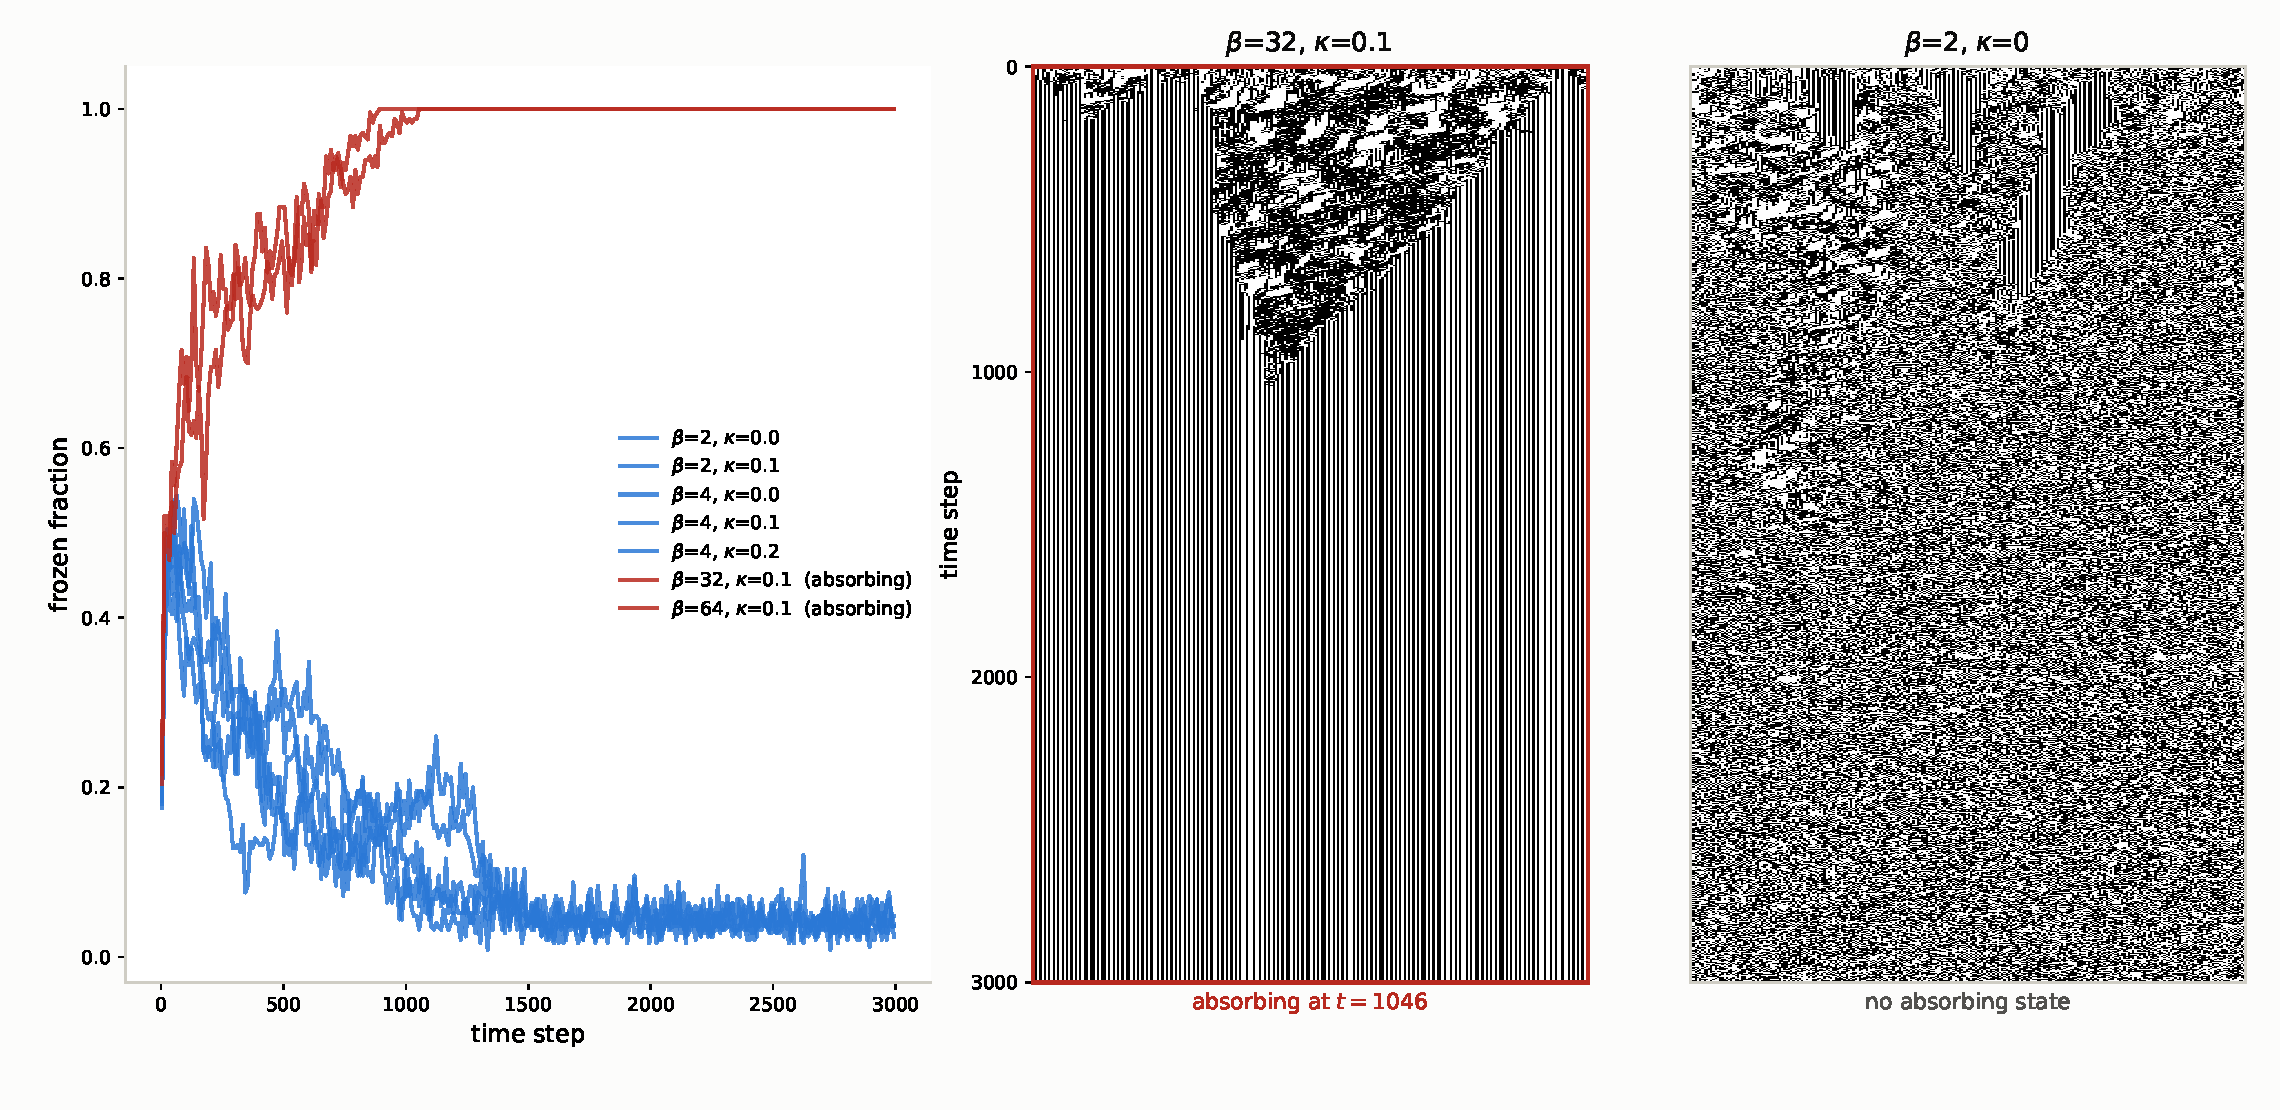
\includegraphics[width=\linewidth]{figures/exo-bifurcation.pdf}
\caption{The two arms of the ridge. Left: frozen fraction against time for the seven
configurations run to $3000$ steps, with the two that reach an absorbing state drawn in
red. The arms separate within the first few hundred steps and do not cross again. Centre
and right: the two extremes as spacetime diagrams --- $\beta = 32$, $\kappa = 0.1$, which
fragments the frozen field for some five hundred steps and is then squeezed out, against
$\beta = 2$, $\kappa = 0$, which erodes the frozen field to nothing and continues. The same
contest, opposite winners.}
\label{fig:exo-bifurcation}
\end{figure}

Two facts about this pair matter more than either alone. First, they are the same
kind of object: both carry coherent propagating structure and sustained genotype
diversity, and they differ in which phase wins. Second, the search objective
ranks them the wrong way round --- $0.625$ for the arm that dies against $0.422$
for the arm that lives. Across the seven configurations run to $3000$ steps on
two seeds the separation is perfect and inverted: every configuration that
reaches an absorbing state scored higher than every configuration that does not.

\subsection{The example in the valley}

Between the two arms the objective falls to its minimum, and it is there that
the most interesting configuration sits. Bisecting $\beta$ between the arms at
$\kappa = 0.1$ locates the crossing between them: $\beta = 12$, $14$ and $16$ all
absorb, at $t = 1917$, $2604$ and $1722$; $\beta = 8$ and $\beta = 10$ do not.

At $\beta = 8$, $\kappa = 0.1$, one realisation sustains an intermediate state
for as long as we have run it. Across three windows spanning $10{,}000$ steps the
frozen fraction reads $0.071$, $0.048$ and $0.073$ --- neither collapsing to the
live-arm value of $0.04$ nor climbing toward one --- with $391$ distinct frozen
regions still forming and dissolving at $t = 9500$ and no absorbing state at any
point. The frozen phase is fine-grained and in continuous turnover: as spacetime
connected components the regions have a median lifetime of $24$ steps and a
median width of $4$ cells, and the largest reaches an area of only $650$, so
no region coarsens into a permanent continent within the observed horizon.

\begin{figure}[htbp]
\centering
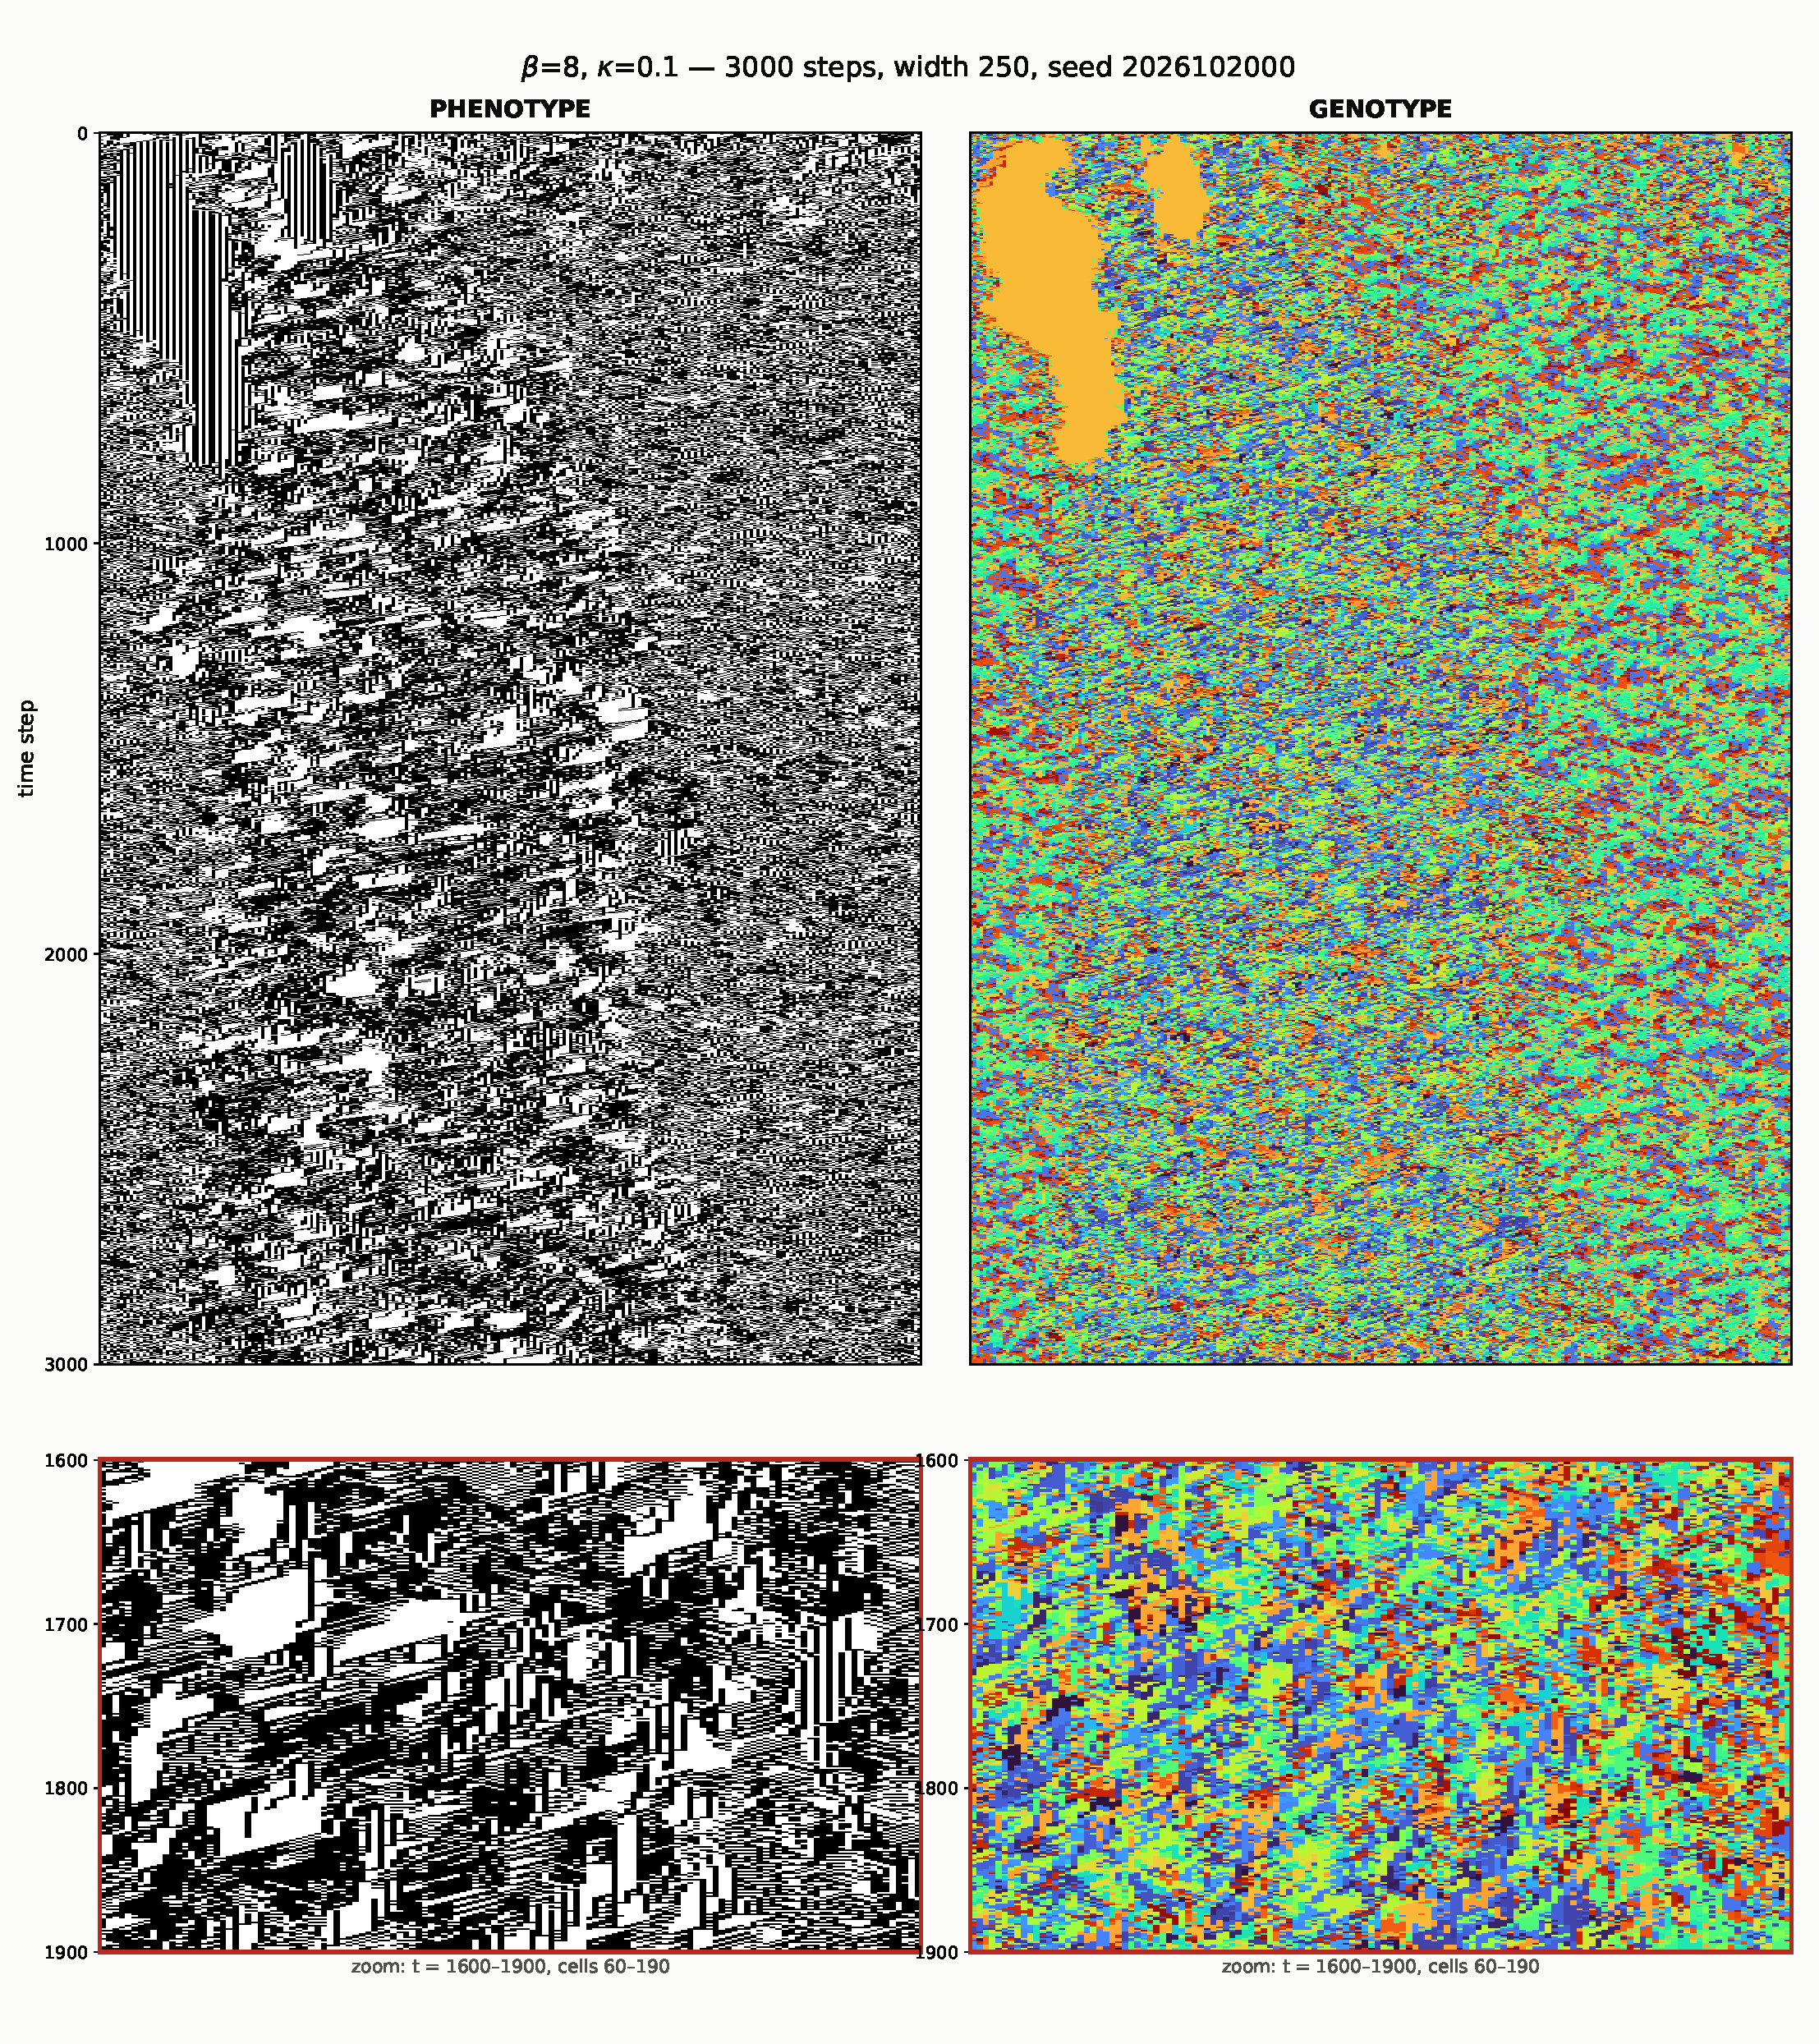
\includegraphics[width=\linewidth]{figures/exo-lavalamp-spacetime.pdf}
\caption{$\beta = 8$, $\kappa = 0.1$, both layers. Coherent diagonal propagating
structure runs the full sheet after the initial transient. The genotype carries
one monoculture region, gone by $t \approx 500$, and thereafter remains diverse
(mean row diversity $0.306$, churn $0.405$ per step, all $256$ sigils present).
The lower row zooms to the scale of the frozen regions, median $4$ cells by $24$
steps.}
\label{fig:exo-lavalamp}
\end{figure}

This configuration is the phenomenon in the third sense distinguished at the
outset---frozen and moving structure coexisting, neither absorbing the other---and so the
one such a search would have been built to find. It is also the one the objective ranks eighth of thirty-five, at
$0.453$, below both arms of its own ridge.

\subsection{What these examples do and do not establish}

The honest description of this region is not that neither phase wins. It is that
\textbf{the parameters do not determine which phase wins.} The second seed at
$\beta = 8$ loses its frozen phase entirely, reading $0.103$, $0.000$ and
$0.001$ across the same three windows. At $\beta = 10$ the two seeds reach
\emph{opposite} outcomes: one sheds its frozen phase to $0.141$, the other
freezes completely and absorbs at $t = 6346$. Widening the lattice to $1000$
cells changes the answer again, and since that run also extended the horizon we
cannot attribute the change to width alone.

Realisation-to-realisation variance dominating a parameter's effect is what a
critical region looks like, and we report it as that rather than as a regime.
What the three examples establish is that this substrate contains configurations
of all three kinds --- one phase winning, the other winning, and neither winning
within the horizon we can afford --- and that they are separated by a bisectable
boundary in $\beta$. What they do not establish is a critical point, which would
require the intermediate behaviour to be a property of the parameters rather than
of the draw, and we have evidence against that at the two points tested.

\begin{figure}[htbp]
\centering
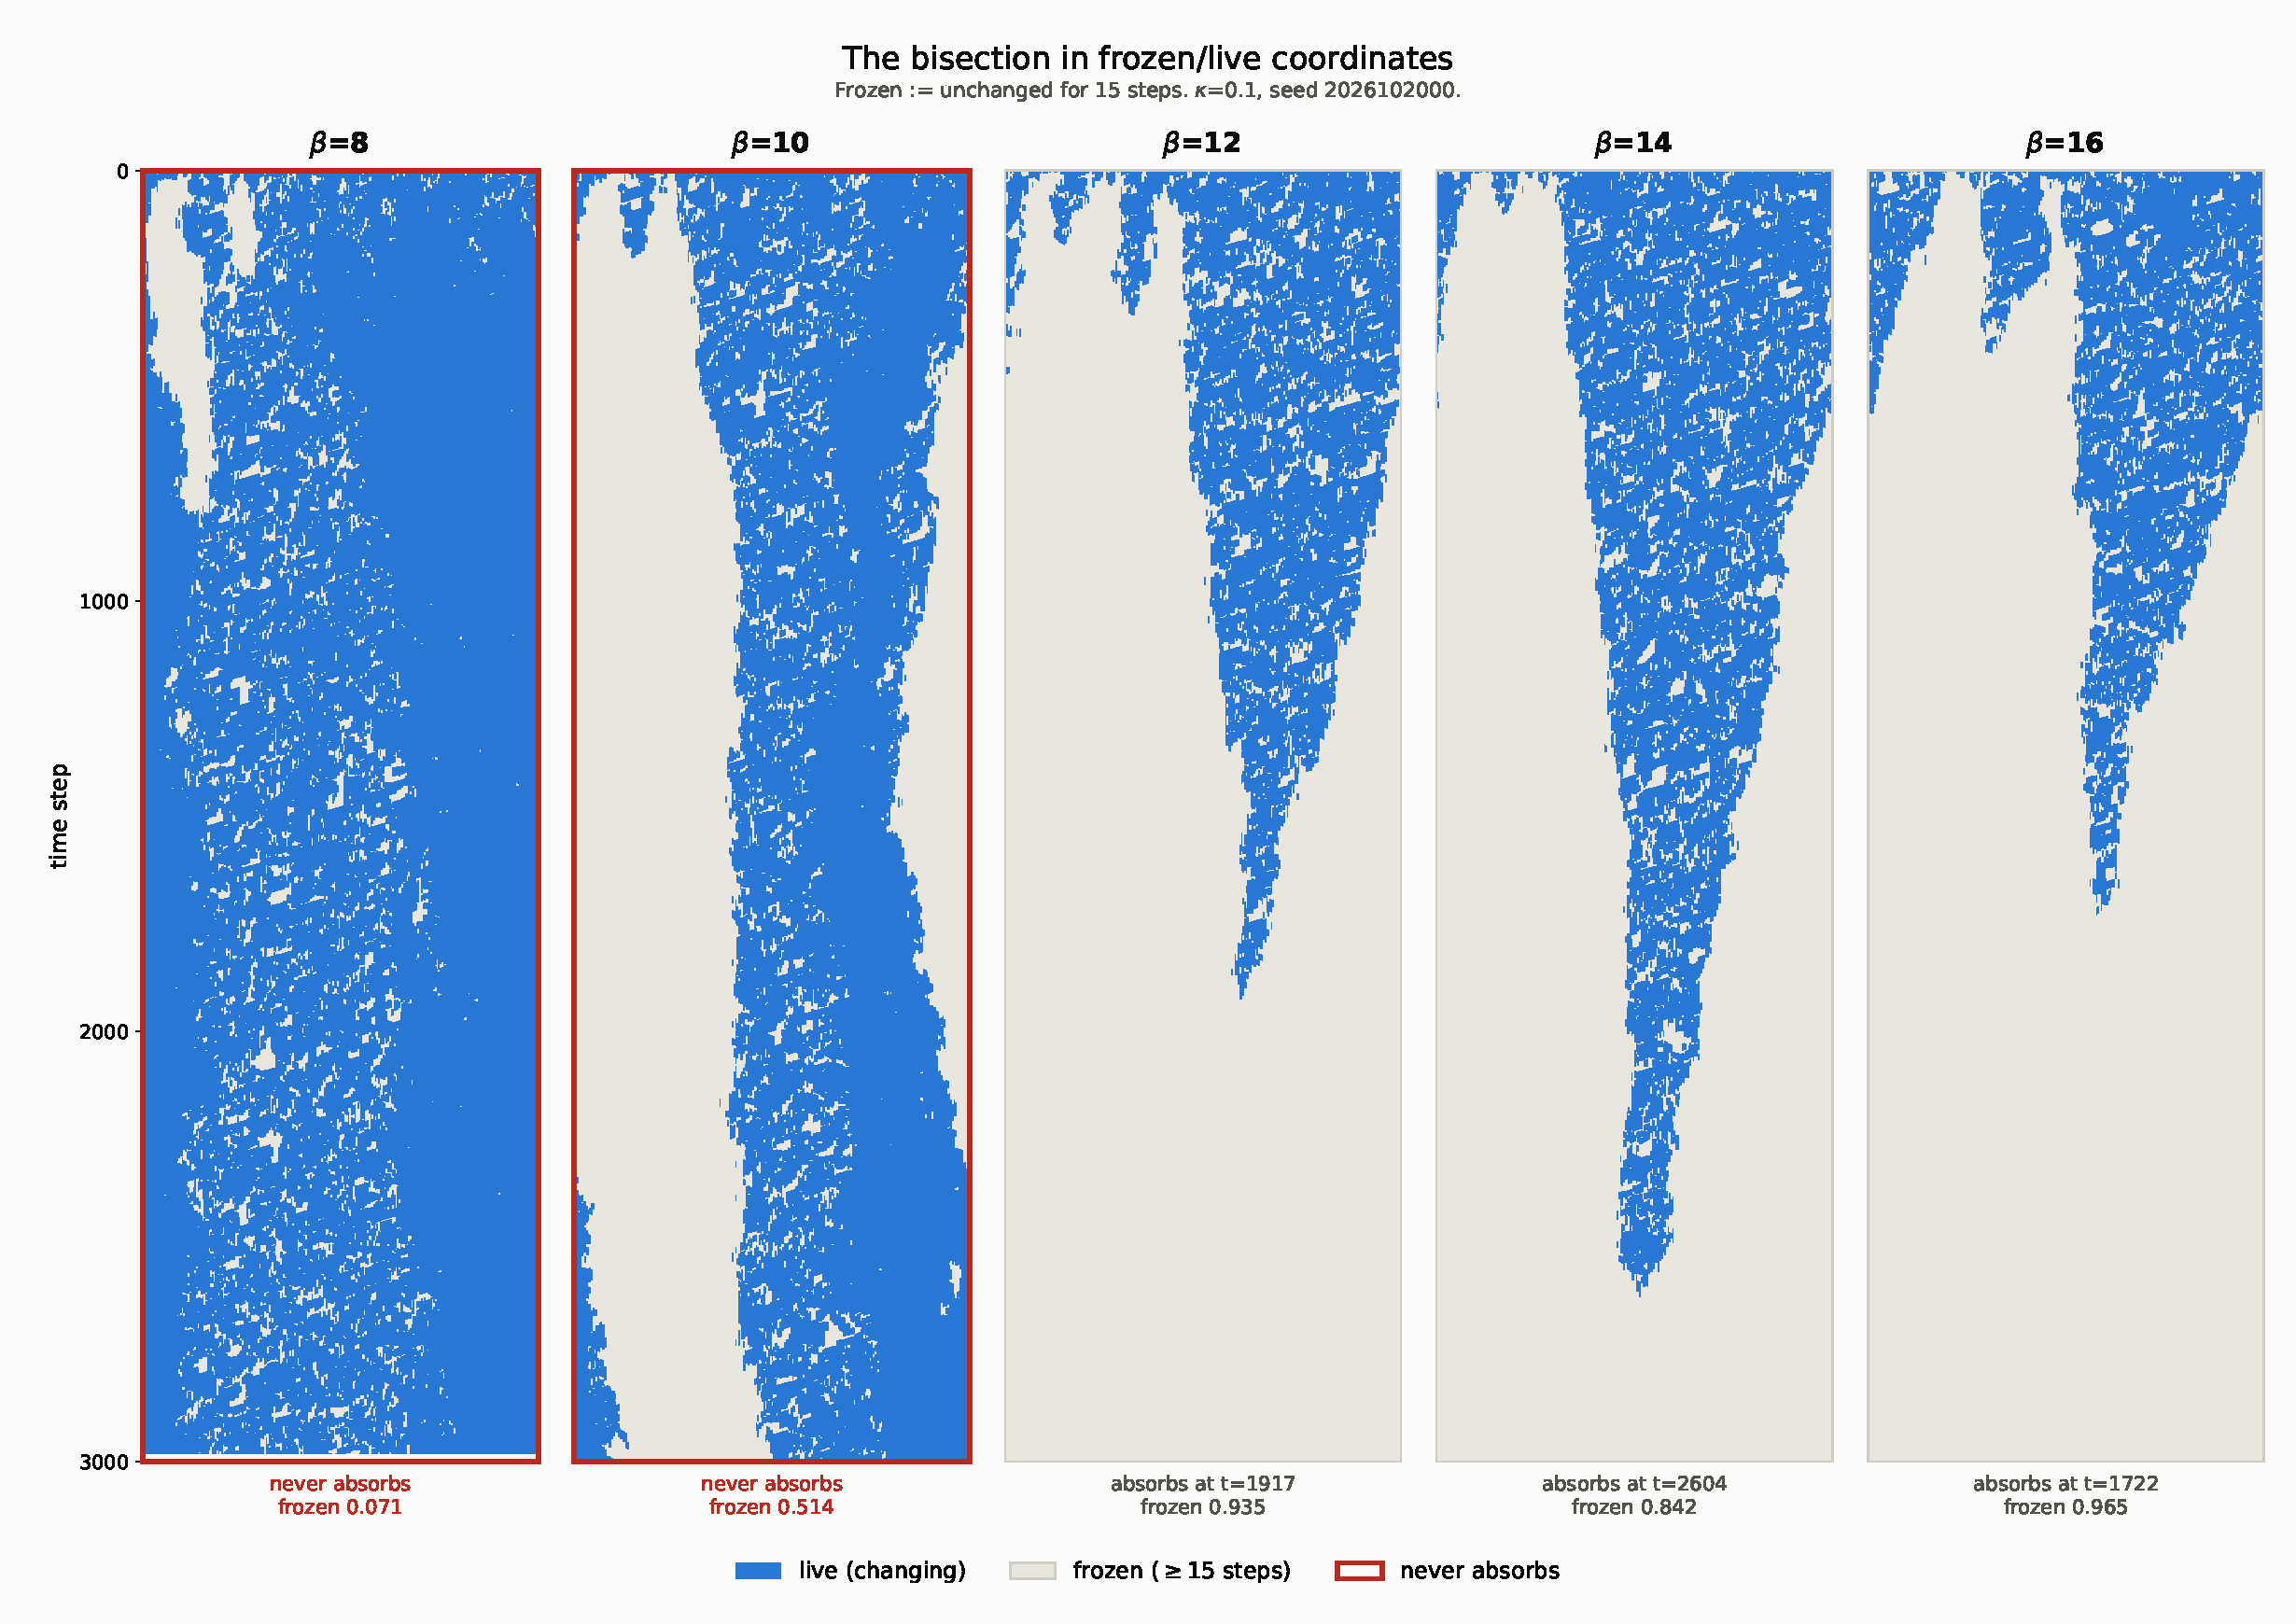
\includegraphics[width=\linewidth]{figures/exo-bisection.pdf}
\caption{The bisection in frozen/live coordinates, $\kappa = 0.1$. Frozen is
defined as unchanged for fifteen steps; at a four-step threshold the median
frozen episode is itself four steps and the turnover count inflates
thirteen-fold. $\beta = 12$, $14$ and $16$ taper to an absorbing state;
$\beta = 8$ and $10$ do not.}
\label{fig:exo-bisection}
\end{figure}

One methodological point generalises beyond these three examples and is the
reason the section is measured by persistence rather than by any of the
alternatives we tried. Every configuration reported here was present in the
thirty-five-cell search of Supplement~5 and was scored there over a $250$-step
window. At that horizon the example in the valley is unremarkable and the arm
that dies looks best. The behaviour that separates them --- absorption at
$t = 1046$, turnover sustained past $t = 9500$ --- occurs entirely outside the
window in which the objective was computed. An instrument validated on
$250$-step reference automata can be measuring a transient in a system whose
transients run four times longer.
